\documentclass[10pt, letterpaper]{report}
% !TeX program = xelatex
%==================PREAMBOLO=======================%
\usepackage[utf8]{inputenc}
\usepackage{psvectorian}
\usepackage{pgfplots}
\usepackage[Rejne]{fncychap}
\usepackage[export]{adjustbox}
\usepackage[T1]{fontenc}
\usepackage{lmodern}
\usepackage{blindtext}
\usepackage{pdfpages}
\usepackage[shortlabels]{enumitem}
\usepackage{moresize}
\usepackage{graphicx} % Required for inserting images
\usepackage{hyperref}
\usepackage{listings}
\usepackage[table,xcdraw]{xcolor}
\usepackage{amssymb}
\usepackage{amsmath}
\usepackage[italian]{babel}
\usepackage{nicefrac, xfrac}
\usepackage{tikz}
\usepackage{tikz-3dplot}
\usepackage{mathrsfs} 
\usepackage{titletoc}
\usepackage{fancyhdr}
\usepackage{psvectorian,lipsum}
\usepackage{fourier-orns}
\usepackage{lipsum}
\usepackage{multicol}
\usepackage[paper=a4paper,left=25mm,right=25mm,bottom=25mm,top=25mm]{geometry}
\definecolor{light-gray}{gray}{0.95}
\definecolor{cop}{HTML}{f7ecd7}
\definecolor{copAut}{HTML}{ababab}
\definecolor{copAut2}{HTML}{c3c3e6}
\definecolor{purcop}{HTML}{d0d3db}
\definecolor{sapienza}{HTML}{660f1d}
\definecolor{lightSapienza}{HTML}{e3d3d5}
\definecolor{darkgreen}{HTML}{008000}
\definecolor{cartaRiciclata}{HTML}{fcfcf7}
\newcommand{\redText}[1]{\color{red}#1\color{black}}
\newcommand{\code}[1]{\colorbox{light-gray}{\texttt{#1}}}
\newcommand{\codee}[1]{\colorbox{white}{\texttt{#1}}}
\newcommand{\K}{{\mathbb K}}
\newcommand{\notimplies}{%
  \mathrel{{\ooalign{\hidewidth$\not\phantom{=}$\hidewidth\cr$\implies$}}}}
\newcommand{\flowerLine}{ \begin{center}\decofourleft\hphantom{ }\decoone\hphantom{ }\decofourright\hphantom{}\hphantom{aa}
\decofourleft\hphantom{ }\decoone\hphantom{ }\decofourright\hphantom{}\hphantom{aa}
\decofourleft\hphantom{ }\decoone\hphantom{ }\decofourright\hphantom{}\hphantom{aa}
\decofourleft\hphantom{ }\decoone\hphantom{ }\decofourright\hphantom{}\hphantom{aa} 
\decofourleft\hphantom{ }\decoone\hphantom{ }\decofourright\hphantom{}\hphantom{aa}
\decofourleft\hphantom{ }\decoone\hphantom{ }\decofourright\hphantom{}\hphantom{aa}
\decofourleft\hphantom{ }\decoone\hphantom{ }\decofourright\hphantom{}\hphantom{aa}
\decofourleft\hphantom{ }\decoone\hphantom{ }\decofourright\hphantom{}\hphantom{aa}
\decofourleft\hphantom{ }\decoone\hphantom{ }\decofourright\hphantom{}\hphantom{aa}
\end{center}}
\definecolor{g}{RGB}{60, 50, 50}
\newcommand{\textg}[1]{\color{g}{\textbf{#1}}\color{black}}
\newcommand{\teo}[1]{{\large\color{sapienza}\textbf{Teorema #1 :\hphantom{a}}}}
\newcommand{\defi}[1]{{\large\color{sapienza}\textbf{Definizione #1 :\hphantom{a}}}}
\newcommand{\claim}[1]{{\color{sapienza}\textbf{Claim #1 :\hphantom{a}}}}
\newcommand{\lemma}[1]{{\color{sapienza}\textbf{Lemma #1 :\hphantom{a}}}}
\newcommand{\dimo}[1]{{\color{sapienza}\textbf{Dimostrazione #1 :\hphantom{a}}}}
\newcommand{\prop}[1]{{\color{sapienza}\textbf{Proposizione #1 :\hphantom{a}}}}
\newcommand\greybox[1]{%
  \vskip\baselineskip%
  \par\noindent\colorbox{light-gray}{%
    \begin{minipage}{\textwidth}#1\end{minipage}%
  }%
  \vskip\baselineskip%
}
\newcommand\sapbox[1]{%
  \vskip\baselineskip%
  \par\noindent\colorbox{lightSapienza}{%
    \begin{minipage}{\textwidth}#1\end{minipage}%
  }%
  \vskip\baselineskip%
}
\newcommand{\ridFunc}{{f:\Sigma^*\rightarrow \Sigma^*}}
\newcommand{\rid}{{\le_m^P}}
\newcommand{\Z}{{\mathbb Z}}
\newcommand{\blank}{{\sqcup}}
\newcommand{\R}{{\mathbb R}}
\newcommand{\N}{{\mathbb N}}
\newcommand{\C}{{\mathbb C}}
\newcommand{\Sn}{{\mathcal S_n}}
\newcommand{\An}{{\mathcal A_n}}
\newcommand{\E}{{\mathcal E}}
\newcommand{\B}{{\mathcal B}}
\newcommand{\mcm}{{\text{mcm}}}
\newcommand{\rg}{{\text{rg}}}
\newcommand{\ve}{{\bar v}}
\newcommand{\spaz}{{\text{\hphantom{aa}}}}
\newcommand{\MCD}{{\text{MCD}}}
\newcommand{\tc}{{\text{ tale che }}}
\newcommand{\supp}{{\text{Supp}}}
\newcommand{\acc}{\\\hphantom{}\\}
\newcommand{\esempio}[1]{{\acc\large\color{sapienza}\textbf{Esempio #1 \hphantom{a}}\acc}}
\newcommand{\bra}[1]{\langle #1 \rangle}
\newcommand{\aut}{{\text{Aut}}}
\newcommand{\Span}{{\text{Span}}}
\newcommand{\End}{{\text{End}}}
\newcommand{\cen}{{\text{Centro}}}
\newcommand{\norm}{{\unlhd}}
\newcommand{\ciclS}{{\left \langle }}
\newcommand{\ciclE}{{\right \rangle }}
\newcommand{\boxedMath}[1]{\begin{tabular}{|c|}\hline \texttt{#1} \\ \hline\end{tabular} :} 
\newcommand{\shell}[1]{\colorbox{black}{\textcolor{white}{\texttt{#1}}}}
\newcommand{\eqImportante}[1]{\begin{center}\huge\lefthand\hphantom{a}
    \normalsize\texttt{#1}
    \hphantom{aaa}\huge\righthand\end{center}}

\fancyhf{}
\pagestyle{fancy}
\usepackage{pgf-pie}  
\usetikzlibrary{positioning}

\renewcommand{\headrule}{%
\vspace{-8pt}\hrulefill
\raisebox{-2.1pt}{\quad\decothreeleft\decotwo\decothreeright\quad}\hrulefill}

%sta roba serve per il codice C
\definecolor{mGreen}{rgb}{0,0.6,0}
\definecolor{mGray}{rgb}{0.5,0.5,0.5}
\definecolor{mPurple}{rgb}{0.58,0,0.82}
\definecolor{backgroundColour}{rgb}{0.95,0.95,0.92}

\lstdefinestyle{CStyle}{
    backgroundcolor=\color{backgroundColour},   
    commentstyle=\color{mGreen},
    keywordstyle=\color{magenta},
    numberstyle=\tiny\color{mGray},
    stringstyle=\color{mPurple},
    basicstyle=\footnotesize,
    breakatwhitespace=false,         
    breaklines=true,                 
    captionpos=b,                    
    keepspaces=true,                 
    numbers=left,                    
    numbersep=5pt,                  
    showspaces=false,                
    showstringspaces=false,
    showtabs=false,                  
    tabsize=2,
    language=C
}
\lstdefinestyle{CppStyle}{
    backgroundcolor=\color{backgroundColour},   
    commentstyle=\color{mGreen}\ttfamily,
    morecomment=[l][\color{magenta}]{\#}
    keywordstyle=\color{blue}\ttfamily,
    numberstyle=\tiny\color{mGray},
    stringstyle=\color{red}\ttfamily,
    basicstyle=\ttfamily,
    breakatwhitespace=false,         
    breaklines=true,                 
    captionpos=b,                    
    keepspaces=true,                 
    numbers=left,                    
    numbersep=5pt,                  
    showspaces=false,                
    showstringspaces=false,
    showtabs=false,                  
    tabsize=2,
    language=C
}
\lstset{language=C++,
                basicstyle=\ttfamily,
                keywordstyle=\color{blue}\ttfamily,
                stringstyle=\color{red}\ttfamily,
                commentstyle=\color{green}\ttfamily,
                morecomment=[l][\color{magenta}]{\#}
}
%fine roba che serve per il codice C
\usepackage{minted}
 %TOGLI COMMENTO SE USI XELATEX
%\usepackage{fontspec}
\title{\jobname} %========TITOLO========%
\author{Marco Casu}
\date{\vspace{-5ex}}
\begin{document}

%==================COPERTINA=======================%
\begin{titlepage}
    \pagecolor{copAut}
\begin{center}
    %TOGLI COMMENTO SE USI XELATEX
   %\setmainfont{Palace Script MT}
   \HUGE Marco Casu\acc
    %\setmainfont{Grand Casino}
     %TOGLI COMMENTO SE USI XELATEX
    %\setmainfont{h Halfroad}
    \HUGE \decothreeleft\hphantom{ }{\fontsize{48}{50}\selectfont \jobname}\hphantom{ }\decothreeright
     %TOGLI COMMENTO SE USI XELATEX
   % \setmainfont{Times New Roman}
\end{center}
\thispagestyle{empty}
\begin{figure}[h]
    \centering{
        %l'immagine deve avere una risoluzione 2048x2048
        \includegraphics[width=1\textwidth ]{images/Copertina.jpeg}
    }
\end{figure}
\vfill 
\centering \includegraphics[width=0.4\textwidth ]{../../../preamble/Stemma_sapienza.png} \acc
\centering \Large \color{sapienza}Facoltà di Ingegneria dell'Informazione,
Informatica e Statistica\\
Dipartimento di Informatica
\end{titlepage}

%===================FINE COPERTINA======================%
\newpage
\pagecolor{cartaRiciclata}%\setmainfont{Algerian}
\Large
Questo documento è distribuito sotto la licenza 
\color{blue}\href{https://www.gnu.org/licenses/fdl-1.3.txt}{GNU}\color{black},  
è un resoconto degli appunti (eventualmente integrati con libri di testo) tratti dalle lezioni del corso di \jobname
\hphantom{a}per la laurea 
triennale in Informatica. Se dovessi notare errori, ti prego di segnalarmeli.\acc 
Nota bene : Essendo questi appunti di un corso esterno alla facoltà di Informatica, 
è presente un capitolo "Complementi" che può risultare utile al lettore.
\newpage %\setmainfont{Times New Roman}
\normalsize
\tableofcontents 
\newpage

%==================FOOTER e HEADER=======================%
\fancyhf{}
\fancyhead[L]{\nouppercase{\leftmark}}
\fancyhead[R]{Sezione \thesection}
\fancyfoot[C]{\thepage}
\fancyfoot[L]{Appunti di \jobname}
\fancyfoot[R]{ Marco Casu}
%\fancyfoot[R]{\setmainfont{Palace Script MT}\huge Marco Casu \setmainfont{Times New Roman}}
%==================FOOTER e HEADER=======================%

%Ricorda del comando \flowerLine per separare le sottosezioni. Le sezioni si separano nelle diverse pagine

%==================INIZIO======================%
\chapter{Complementi}
\section{La Trasformata di Laplace} 
La trasformata di Laplace è una \textit{trasformata integrale}, nello specifico, è una 
funzione che associa ad una funzione di variabile reale, una funzione di variabile 
complessa.\acc 
\defi{(Trasformata di Laplace)} : Sia $f$ una funzione di variabile reale, nulla 
in $(-\infty,0)$, si chiama trasformata di Laplace di $f$ la funzione 
$$ \mathcal{L}[f](p)=\int_0^{+\infty} e^{-px}f(x)\ dx \ \ \ \ p\in \C$$
Essendo $p = \alpha + i\beta$ una variabile complessa, la funzione integranda si può riscrivere 
$$\int_0^{+\infty} e^{-px}f(x)\ dx = 
\int_0^{+\infty} e^{-(\alpha + i\beta)x}f(x)\ dx$$
Ricordando l'identità di Eulero $$ e^{ix}=\cos(x)+i\sin(x)$$
Si ha 
\begin{eqnarray}
    e^{-(\alpha + \beta i)x} = e^{-\alpha x}\cdot e^{-\beta i x} =\\ 
    e^{-\alpha x}\cdot \Big(
    \cos(-\beta x)+ i \sin(-\beta x)    
    \Big) = e^{-\alpha x}\cdot \Big(
        \cos(\beta x)- i \sin(\beta x)    
        \Big) = \\ 
        e^{-\alpha x}\cos(\beta x)- i e^{-\alpha x}\sin(\beta x)
\end{eqnarray}
Quindi $$ \mathcal{L}[f](p)=\mathcal{L}[f](\alpha + i\beta)=
\int_0^{+\infty} e^{-(\alpha + i\beta)x}f(x)\ dx=
$$
$$
\int_0^{+\infty} e^{-\alpha x}\cos(\beta x)f(x)-ie^{-\alpha x}\sin(\beta x)f(x)\ dx =$$
$$ 
\int_0^{+\infty} e^{-\alpha x}\cos(\beta x)f(x)\ dx-i\int_0^{+\infty}e^{-\alpha x}\sin(\beta x)f(x)\ dx
$$
Se l'integrale $\mathcal{L}[f](\alpha + i\beta)$ converge per un certo
 $\alpha \in \R$, allora converge per $p = \alpha + i\beta$ per ogni altro $\beta \in \R$. Se per 
 $f$ esiste almeno un $p\in\C$ tale che $\mathcal{L}[f](p)<\infty$, allora $f$ si dice 
 \textit{trasformabile secondo Laplace}.\acc
 In generale, se $\mathcal{L}[f](p)<\infty$ per $p=p_0$, allora è definita anche nel semipiano 
 complesso $$\{p\in \C \ |\ \Re(p)>\Re(p_0)\}$$
 Sia $\alpha_0$ l'estremo inferiore dell'insieme $\{\alpha \in \R \ |\ \mathcal{L}[f](p)<\infty\land \Re(p)>\alpha\}$, allora 
 il semipiano $\{p\in \C \|\ \Re(p)>\alpha_0\}$ è detto \textbf{semipiano di convergenza}.
 \begin{center}
    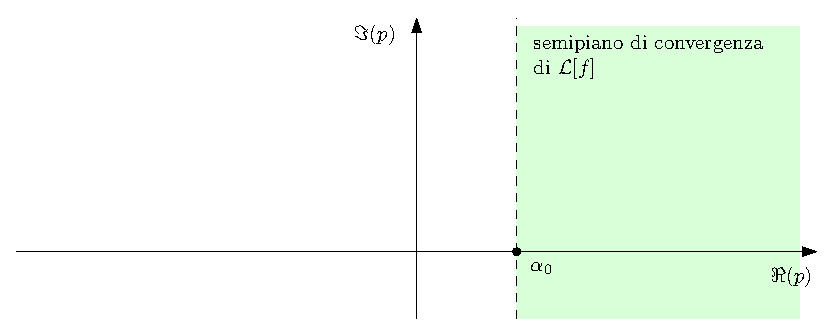
\includegraphics[width=0.6\textwidth ]{images/semiPianoConv.eps}
 \end{center}
 Vediamo un esempio di trasformata, si consideri $$ 
 H(x)=\begin{cases}
    1 \text{ se }x\ge 0\\ 0 \text{ altrimenti }
 \end{cases}
 $$
 \begin{center}
 \begin{figure}[h!]
    \centering
    \begin{tikzpicture}[scale=0.7, transform shape]
        \begin{axis}[
        ymin=-3,
        ymax = 3,
        xmin=-3,
        xmax = 3,
        axis lines = center,
        xtick distance=1, ytick distance=1,
        grid style=dashed,
        ymajorgrids=true,
        xmajorgrids=true,
        xlabel = \(\),
        ylabel = {\(\)},
        ]
        %Below the red parabola is defined
        \addplot [
        domain=0:3,
        samples=20,
        color=blue,
        ]
        {1};
        \end{axis}
        \end{tikzpicture}
        \caption{Funzione di Heaviside}
\end{figure}
\end{center}
Si calcola 
$$ \mathcal{L}[H](p)=\int_0^{+\infty}e^{-px}\cdot 1 \ dx = 
\lim_{T\rightarrow+\infty}\mathcal{L}[H](p)=\int_0^{T}e^{-px}\cdot 1 \ dx = 
\lim_{T\rightarrow+\infty}\begin{bmatrix}
    -\dfrac{e^{-px}}{p}
\end{bmatrix}_0^T=$$
$$\lim_{T\rightarrow+\infty} -\dfrac{e^{-pT}}{p} - \Big[-\dfrac{e^{-p0}}{p}\Big] =  
\lim_{T\rightarrow+\infty} -\dfrac{e^{-pT}}{p} +\dfrac{1}{p}=\frac{1}{p}$$
Il cui semipiano di convergenza risulta essere $\Re(p)>0$.
\subsection{Proprietà della Trasformata}
\subsubsection{Linearità}
La trasformazione di Laplace gode della proprietà di \textit{linearità}, siano $f(p)$ e $g(p)$ due funzioni 
trasformabili, siano $\lambda,\mu \in \C$ due costanti complesse, se la funzione 
$\lambda \cdot f(p)+\mu \cdot g(p)$ è trasformabile, allora 
$$ 
\mathcal{L}[\lambda \cdot f+\mu \cdot g](p)=\lambda\mathcal{L}[f](p)+\mu\mathcal{L}[g](p)
$$
Il semipiano di convergenza sarà uguale all'intersezione dei due semipiani di convergenza delle funzioni 
di partenza, più precisamente se \begin{itemize}
    \item $f$ ha come semipiano di convergenza $\Re(p)>\alpha$
    \item $g$ ha come semipiano di convergenza $\Re(p)>\beta$
    \item allora $\lambda \cdot f+\mu \cdot g$ ha come semipiano di convergenza $\Re(p)>\max\{\beta,\alpha\}$
\end{itemize}
\subsubsection{Ritardo}
Sia $f$ una funzione trasformabile, si consideri una costante reale $a>0$, la funzione $g(x)=f(x-a)$ è detta 
funzione \textit{ritardata}.\begin{center}
\begin{figure}[h!]\centering
    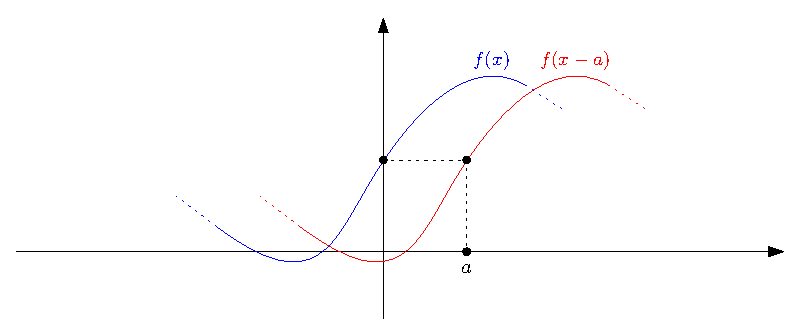
\includegraphics[width=0.6\textwidth ]{images/funRit.eps}
    \caption{funzione ritardata}
 \end{figure}\end{center}
Per il calcolo della trasformata di $g(x)=f(x-a)$ si considera il cambio di variabile $$\begin{matrix}
    t=x-a\\ x=t+a
\end{matrix} $$
Si ricordi come, se $f$ è nulla in $(-\infty,0)$, allora $g$ sarà nulla in $(0,a)$.
$$ 
\mathcal{L}[g](p)=\int_0^{+\infty}e^{-px}g(x)\ dx =\int_a^{+\infty}e^{-px}f(x-a)\ dx  =
\int_a^{+\infty}e^{-p(t+a)}f(t)\ dx = 
$$ 
$$ 
\int_a^{+\infty}e^{-pt-pa}f(t)\ dx 
= \int_a^{+\infty}e^{-pt}e^{-pa}f(t)\ dx = e^{-pa}\int_a^{+\infty}e^{-pt}f(t)\ dx = 
e^{-pa}\mathcal{L}[f](p)$$
Dunque si ricavano le cosiddette \textit{formule del ritardo} : 
$$ 
\mathcal{L}[f(x-a)](p)=e^{-pa}\mathcal{L}[f(x)](p)
$$ $$ 
\mathcal{L}[e^{ax}f(x)](p)=\mathcal{L}[f](p-a)
$$
\subsubsection{Trasformazione di una derivata e di una primitiva}
La seguente proprietà risulta cruciale nell'utilizzo della trasformata di Laplace per la risoluzione di 
equazioni differenziali. Le dimostrazioni dei seguenti risultati non saranno trattate in quanto non 
sono argomento di questo corso.\acc 
Sia $f$ una funzione derivabile, la cui derivata è continua in $[0,\infty)$. Sia inoltre $f'$ trasformabile, con 
semipiano di convergenza $\Re(p)>\alpha$, allora anche $f$ è trasformabile, ha semipiano di 
convergenza $\Re(p)>\max\{\alpha,0\}$, e vale la seguente identità :
\eqImportante{$
\mathcal{L}[f'](p)=p\mathcal{L}[f](p)-f(0)
$}
Si generalizza per derivate di ordine maggiore 
$$ 
\mathcal{L}[f''](p)=p^2\mathcal{L}[f](p)-pf(0)-f'(0)
$$
Analogamente, sia $F(x)=\int_0^x f(t)\ dt$, se $f$ è trasformabile ed ha semipiano di convergenza  $\Re(p)>\alpha$, 
allora anche $F$ lo è, ha semipiano di convergenza $\Re(p)>\max\{\alpha,0\}$ e vale che 
\eqImportante{$
\mathcal{L}[F](p)=\dfrac{1}{p}\mathcal{L}[f](p)
$}
\end{document}